% Copyright The Zephyr Project Contributors
% SPDX-License-Identifier: Apache-2.0
%
% Build: pdflatex collision-detection.tex (twice, for the references).
% Figures: tools/make_figures.py doc/figures <collision.csv> <stop.csv> <spin.csv> --events ...

\documentclass[11pt,a4paper]{article}

\usepackage[T1]{fontenc}
\usepackage{lmodern}
\usepackage{amsmath,amssymb,bm}
\usepackage{siunitx}
\usepackage{graphicx}
\usepackage{color}
\usepackage{array,tabularx,longtable}
\usepackage[colorlinks=true,linkcolor=blue,urlcolor=blue,citecolor=blue]{hyperref}

% A4 with 25 mm margins (the geometry package is not installed here).
\setlength{\textwidth}{160mm}
\setlength{\textheight}{237mm}
\setlength{\oddsidemargin}{\dimexpr 25mm - 1in\relax}
\setlength{\evensidemargin}{\oddsidemargin}
\setlength{\topmargin}{\dimexpr 20mm - 1in\relax}
\setlength{\headheight}{0pt}
\setlength{\headsep}{0pt}
\setlength{\footskip}{12mm}
\setlength{\parindent}{0pt}
\setlength{\parskip}{0.55em}
\renewcommand{\arraystretch}{1.18}
\sisetup{per-mode=symbol}
% Let figures sit close to the text that refers to them.
\renewcommand{\topfraction}{0.9}
\renewcommand{\bottomfraction}{0.8}
\renewcommand{\textfraction}{0.07}
\renewcommand{\floatpagefraction}{0.75}
\setcounter{topnumber}{3}
\setcounter{totalnumber}{4}

\newcommand{\g}{\,\mathrm{g}}
\newcommand{\gu}{\mathrm{g}}
\newcommand{\code}[1]{\texttt{#1}}
\newcommand{\azf}{a_{25}}
\newcommand{\vib}{\mathit{vib}}

\title{\textbf{Collision Detection on a Skid-Steer Robot\\with a Single Accelerometer}\\[0.4em]
       \large Method, Physics and Evaluation}
\author{Javad Rahimipetroudi}
\date{21 October 2026 \quad---\quad firmware 0.9.0}

\begin{document}

\maketitle

\begin{abstract}
A four-wheel skid-steer robot (ESP32, Zephyr RTOS) detects collisions with one three-axis
accelerometer sampled at \SI{400}{\hertz}, combined with what the robot knows about its own
motion: the drive command and the actual side speeds. Two features are computed on every
sample: the horizontal acceleration averaged over \SI{25}{\milli\second}, $\azf$, which
captures the one-sided push of an impact while averaging out vibration, and the vibration
energy over \SI{100}{\milli\second}, $\vib$. A collision is reported when a feature crosses its
threshold while the robot is driving; braking, which reaches similar values, is excluded
because it happens after the sides have stopped, and turning, which shakes the robot as hard
as a soft collision, uses its own threshold on $\azf$ only. On 34 recorded events the method
detects all 5 collisions, from a shoe to a box, and raises no alarm on 23 stops and 5 spins;
the motors stop \SIrange{5}{15}{\milli\second} after contact. A second detector derives its
context from the IMU alone, for vehicles whose drive is not accessible, and reaches the same
result on these recordings with thinner margins. The document derives each step
from the physics, gives every formula and constant of the implementation, and states the
limits of the evidence.
\end{abstract}

\tableofcontents

% ---------------------------------------------------------------------------------------
\section{Problem}

A collision and a hard stop both decelerate the robot. A single acceleration threshold cannot
separate them, and on a skid-steer robot it cannot separate either of them from driving:
\begin{itemize}
  \item driving straight at full speed, single samples reach $\pm1$ to $\pm2\g$ of vibration;
  \item a stop from full speed reaches $0.75\g$ averaged over \SI{25}{\milli\second};
  \item a spin shakes the chassis with up to $1.6\g$ of vibration, more than a soft collision.
\end{itemize}
The method therefore combines two features that react differently to impacts and vibration
with the context the robot knows from its own commands: a deceleration while the robot is told
to keep driving is unexpected; the same deceleration right after a stop command is not.

\textbf{Platform.} ESP32-WROOM, Zephyr RTOS; four geared DC motors, two per side, driven by PWM
with a soft start (ramp from 35\,\% to 100\,\% in \SI{0.6}{\second}); GY-85 module with an
ADXL345 accelerometer and an ITG3205 gyroscope on I\textsuperscript{2}C, mounted rigidly near
the centre with $x$ pointing forward. The source files are \code{src/collision.c},
\code{src/imu.c} and \code{tools/analyze.py}.

% ---------------------------------------------------------------------------------------
\section{Physical background}

\subsection{Collision versus braking}

Both events take the robot from its speed $v$ to rest. By Newton's second law the mean
acceleration over the change is
\begin{equation}
  \bar a = \frac{\Delta v}{\Delta t}.
\end{equation}
At full power the robot drives at about $v = \SI{0.3}{\metre\per\second}$
(\SIrange{0.27}{0.35}{\metre\per\second}, integrated from the recorded acceleration). The two
events differ in $\Delta t$:
\begin{itemize}
  \item \textbf{Braking.} When the drive stops, the PWM inputs go to zero and the gear motors
    coast; rolling resistance and gearbox friction stop the robot. The recordings show a mean of
    $0.26$ to $0.28\g$ over \SI{100}{\milli\second}, hence
    $\Delta t = 0.3 / (0.27 \cdot 9.81) \approx \SI{0.11}{\second}$.
  \item \textbf{Collision.} The obstacle stops the robot within the deformation of the contact.
    A mean of $1.0$ to $1.8\g$ gives $\Delta t = 0.3 / ((1.0\ldots1.8) \cdot 9.81) \approx$
    \SIrange{17}{31}{\milli\second}.
\end{itemize}
A collision is the same change of velocity in a quarter to a sixth of the time, and therefore a
several times larger acceleration over a short window.

\subsection{Contact model}

Modelling the contact as a spring of stiffness $k$ acting on the robot's mass $m$ gives a half
sine pulse with
\begin{equation}
  a_\text{peak} = v\,\sqrt{\frac{k}{m}}, \qquad
  t_\text{contact} = \pi\,\sqrt{\frac{m}{k}}, \qquad
  a_\text{peak}\, t_\text{contact} = \pi\, v .
\end{equation}
The product is fixed by the speed: a hard obstacle (large $k$) gives a short, high pulse, a soft
one a longer, lower pulse. The measurements follow this: the shoe produced $1.0\g$, the box
$1.7$ to $1.8\g$. The averaging window must therefore be about as long as the contact, tens of
milliseconds: long enough to average out vibration, short enough not to dilute the impact with
the time before and after it.

\subsection{Vibration and averaging}

The chassis vibrates from the gearboxes, the wheels and the floor. Its acceleration oscillates
and is close to zero-mean over a few milliseconds, unlike the one-sided push of an impact.
Averaging $N$ samples of uncorrelated vibration reduces its RMS by $\sqrt{N}$, by about 3 for
$N=10$. The moving average is a low-pass filter with the amplitude response
\begin{equation}
  |H(f)| = \left| \frac{\sin(\pi f N / f_s)}{N \sin(\pi f / f_s)} \right| ,
\end{equation}
whose first zero lies at $f_s/N$: \SI{40}{\hertz} for $N=10$ at $f_s=\SI{400}{\hertz}$
(Figure~\ref{fig:response}). Vibration above about \SI{40}{\hertz} is strongly attenuated, while
an impact of \SI{25}{\milli\second} or longer passes almost entirely. What the average removes
becomes the second feature: the high-frequency energy, which rises sharply when the robot hits
something rigid and keeps pushing.

\begin{figure}[!htbp]
  \centering
  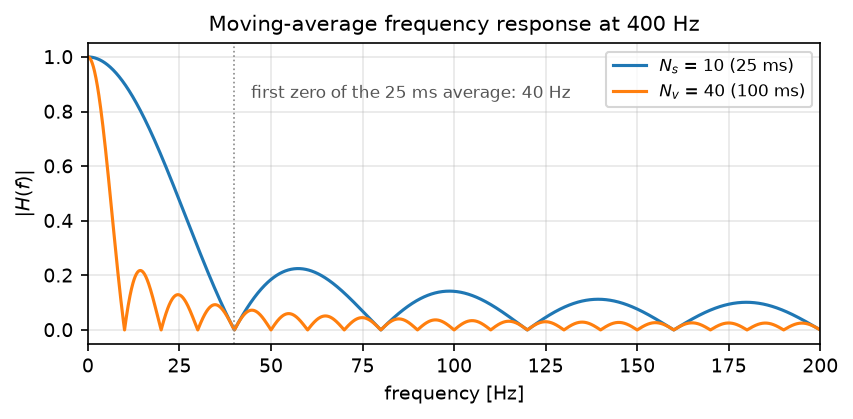
\includegraphics[width=0.9\linewidth]{figures/response.png}
  \caption{Amplitude response of the \SI{25}{\milli\second} and \SI{100}{\milli\second} moving
    averages at \SI{400}{\hertz}.}
  \label{fig:response}
\end{figure}

\subsection{Turning}

A skid-steer robot turns by driving its sides at different speeds. Its wheels cannot roll in
the direction of the turn, so they slide sideways; the sliding friction, about $\mu N$ per wheel,
alternates between sticking and slipping and excites the chassis over a wide band. A spin on
this robot produced up to $1.64\g$ of vibration, more than the softest collision ($1.17\g$).
The centripetal acceleration of the turn itself is negligible: at the measured spin rate
$\omega \approx \SI{35}{\degree\per\second} = \SI{0.61}{\radian\per\second}$ and a sensor
$r = \SI{0.1}{\metre}$ from the centre of rotation,
\begin{equation}
  a_c = \omega^2 r = 0.37 \cdot 0.1 = \SI{0.037}{\metre\per\second\squared} \approx 0.004\g .
\end{equation}
Turning therefore raises the vibration but hardly the averaged acceleration. This is why the
turning rule drops the vibration feature and keeps a higher threshold on the averaged
acceleration.

\subsection{Direction of a hit}

The obstacle pushes the robot away from itself (Newton's third law), so the robot's
acceleration $\bm a = \bm F / m$ points away from the obstacle. The obstacle lies opposite to the
acceleration:
\begin{equation}
  \theta_\text{obstacle} = \operatorname{atan2}(-a_y, -a_x),
\end{equation}
with $x$ forward, $y$ to the left and $\theta$ counter-clockwise from the front.

% ---------------------------------------------------------------------------------------
\section{Signal chain}

\subsection{Sensor}

The ADXL345 runs at $\pm16\g$ in full-resolution mode: \SI{3.9}{\milli\gu} per count, 13 bits,
$\pm4096$ counts. The output data rate is \SI{400}{\hertz} nominal (measured \SI{392}{\hertz},
\SI{2.55}{\milli\second} sample spacing, within the sensor's clock tolerance), the output
bandwidth $f_s/2 = \SI{200}{\hertz}$. Each sample is timed by the sensor's data-ready interrupt
($t$ in microseconds since boot); the ITG3205 ($\pm\SI{2000}{\degree\per\second}$,
\SI{188}{\hertz} low-pass, 14.375 counts per \si{\degree\per\second}) is read right after it. The
noise at rest is about \SI{5}{\milli\gu} RMS per axis.

\subsection{Plausibility}

A raw reading beyond $\pm4096$ counts ($16\g$) cannot come from the sensor at this range; it is
a corrupted I\textsuperscript{2}C read, observed once as $57.9\g$ and caused by electrical noise
from the motors. Such a sample is discarded and counted:
\begin{equation}
  \text{discard if } |r_x| > 4096 \ \lor\ |r_y| > 4096 \ \lor\ |r_z| > 4096 .
\end{equation}

\subsection{Calibration}

A reading is $r = o + s\,a$ with zero-$g$ offset $o$ and scale $s$. Resting the robot level and
then upside down applies $a = -1\g$ and $+1\g$ to the vertical axis:
\begin{equation}
  o = \frac{r_+ + r_-}{2}, \qquad s = \frac{r_+ - r_-}{2\g} .
\end{equation}
On this module the $z$ axis read $-0.846\g$ and $+1.148\g$: $o = +0.151\g$, $s = 0.997$. The
scale is within 0.3\,\% and left at 1; the offsets (\SI{14}{}, \SI{0}{}, \SI{151}{\milli\gu} on
$x, y, z$) are subtracted in counts, $\text{ofs} = \text{mg} \cdot 1000 / 3900$.

The gyroscope bias drifts with temperature and is measured whenever the robot rests. After the
motors have been stopped for 400 samples (\SI{1}{\second}), 512 samples (\SI{1.3}{\second}) are
averaged and the mean becomes the bias, unless a sample differs from the current bias by more
than \SI{3}{\degree\per\second} (the robot is moved by hand), which restarts the average. The
bias is kept in counts times 16 for sub-count resolution.

\subsection{Robot frame}

On this robot both chips have $x$ forward, $y$ right and $z$ down. They are turned into the frame
of ROS REP-103 ($x$ forward, $y$ left, $z$ up) by negating $y$ and $z$ of both sensors. At rest
the accelerometer reads $+1\g$ on $z$ and a left turn gives a positive yaw rate. The features use
the horizontal components $a_x$ and $a_y$ only.

% ---------------------------------------------------------------------------------------
\section{Features}

Notation: $n$ is the sample index, $a_x[n]$ and $a_y[n]$ the calibrated horizontal acceleration,
$N_s = 10$ (\SI{25}{\milli\second}) and $N_v = 40$ (\SI{100}{\milli\second}) the window lengths
at \SI{400}{\hertz}.

\subsection{Tilt offset}

On a slope the accelerometer measures a component of gravity, $\gu \sin(\text{tilt})$, about
\SI{17}{\milli\gu} per degree. It is learned while the robot does not move and subtracted. The
firmware uses an exponential average with a time constant of 256 samples (\SI{0.64}{\second}):
\begin{equation}
  o_x \leftarrow o_x + \frac{a_x - o_x}{256} \quad \text{while } \text{left} = \text{right} = 0,
  \qquad a'_x = a_x - o_x ,
\end{equation}
and the same for $y$. The analysis tool uses the median of $a_x$ over all samples at rest.

\subsection{Averaged acceleration $\azf$}

\begin{equation}
  m_x[n] = \frac{1}{N_s} \sum_{k=0}^{N_s-1} a'_x[n-k], \qquad
  m_y[n] = \frac{1}{N_s} \sum_{k=0}^{N_s-1} a'_y[n-k], \qquad
  \azf[n] = \sqrt{m_x[n]^2 + m_y[n]^2} .
\end{equation}

\subsection{Vibration $\vib$}

The RMS over the last \SI{100}{\milli\second} of what the \SI{25}{\milli\second} average leaves
out:
\begin{equation}
  \vib[n] = \sqrt{ \frac{1}{N_v} \sum_{k=0}^{N_v-1}
    \Big[ \big(a'_x[n-k] - m_x[n-k]\big)^2 + \big(a'_y[n-k] - m_y[n-k]\big)^2 \Big] } .
\end{equation}

\subsection{Computation on the robot}

The firmware keeps running sums over ring buffers, so each sample costs a few additions and
multiplications whatever the window length:
\begin{align}
  S_x &\leftarrow S_x + a'_x[n] - a'_x[n-N_s], & m_x &= S_x / N_s, \\
  Q   &\leftarrow Q + q[n] - q[n-N_v], & q[n] &= (a'_x - m_x)^2 + (a'_y - m_y)^2, \\
  \azf^2 &= m_x^2 + m_y^2, & \vib^2 &= Q / N_v .
\end{align}
All values are in sensor counts. Comparisons are made on squares against squared thresholds,
$\text{thr}_\text{counts} = \text{thr}_\text{mg} \cdot 1000 / 3900$, so no square root is taken
per sample. The first 100 samples (\SI{250}{\milli\second}) after boot fill the windows and are not
evaluated.

% ---------------------------------------------------------------------------------------
\section{Context and decision rule}

\subsection{Context}

Each sample carries the drive state: the commanded throttle and turn and the actual left and
right side speeds, which include the ramp and the coast before a reversal. From it:
\begin{align*}
  \text{moving}    &= (\text{left} \ne 0) \lor (\text{right} \ne 0), \\
  \text{commanded} &= (\text{throttle} \ne 0) \lor (\text{turn} \ne 0), \\
  t_\text{start}   &= \text{time of the last change of }
                      \big(\operatorname{sign}(\text{left}), \operatorname{sign}(\text{right})\big)
                      \text{ while moving}, \\
  \text{driving}   &= \text{moving} \land \text{commanded} \land (t - t_\text{start} \ge
                      \SI{0.8}{\second}), \\
  \text{turning}   &= \text{driving} \land (\text{turn} \ne 0), \qquad
  \text{straight}   = \text{driving} \land (\text{turn} = 0).
\end{align*}
The \SI{0.8}{\second} after a start or a reversal are excluded: the ramp and the coast shake the
robot without a collision. When the robot stops itself (auto-stop, an inhibit, the coast before
a reversal) the sides are zero and the robot is not driving, even if the command is still
active. The analysis tool further labels samples that are not driving as \emph{starting},
\emph{stopping} (\SI{0.6}{\second} after the command went to stop) or \emph{idle}.

\subsection{Decision rule}

A collision is detected at sample $n$ when
\begin{equation}
  \big[\,\text{straight} \land (\azf > A \lor \vib > V)\,\big]
  \ \lor\
  \big[\,\text{turning} \land (\azf > A_t \lor (V_t > 0 \land \vib > V_t))\,\big] .
\end{equation}

\begin{table}[!htbp]
  \centering
  \begin{tabular}{l l l}
    \hline
    Threshold & Default & Kconfig \\
    \hline
    $A$, straight   & $0.6\g$  & \code{CONFIG\_ROBOT\_COLLISION\_A25\_MG} \\
    $V$, straight   & $0.9\g$  & \code{CONFIG\_ROBOT\_COLLISION\_VIB\_MG} \\
    $A_t$, turning  & $1.0\g$  & \code{CONFIG\_ROBOT\_COLLISION\_A25\_TURN\_MG} \\
    $V_t$, turning  & off (0)  & \code{CONFIG\_ROBOT\_COLLISION\_VIB\_TURN\_MG} \\
    \hline
  \end{tabular}
  \caption{Thresholds. At run time the link command \code{T A V [A\_t V\_t]} (in mg) changes
    them.}
  \label{tab:thresholds}
\end{table}

The values follow from the evaluation (Section~\ref{sec:evaluation}): driving straight stays
below $0.12\g$ $\azf$ and $0.61\g$ $\vib$ (99th percentiles), collisions start at $1.0\g$ and
$1.17\g$; turning reaches $0.67\g$ $\azf$ and $1.64\g$ $\vib$, so only $\azf$ separates there.
Braking is excluded by the context, not by the thresholds: its jolt comes after the sides went
to zero.

% ---------------------------------------------------------------------------------------
\section{Response and latency}

The mode is set by \code{CONFIG\_ROBOT\_COLLISION\_MODE} or the link command \code{M}:
\textbf{stop} (2, default) sets the drive inhibit at the detecting sample, which sets both sides
to zero immediately and blocks drive commands until a reset; \textbf{monitor} (1) reports the
collision and keeps driving, at most once per second; \textbf{off} (0).

The 40 samples (\SI{100}{\milli\second}) after detection characterise the event. The direction
comes from the first 8 samples (\SI{20}{\milli\second}), the contact itself, because the robot may
push and shake afterwards:
\begin{equation}
  \theta = \operatorname{atan2}\!\Big(-\sum_{k=1}^{8} m_y[n+k],\ -\sum_{k=1}^{8} m_x[n+k]\Big),
  \qquad
  \text{sector} = \left\lfloor \frac{\theta + 22.5^\circ}{45^\circ} \right\rfloor \bmod 8,
\end{equation}
with sectors 0 front, 1 front-left, 2 left, 3 back-left, 4 back, 5 back-right, 6 right,
7 front-right. The strength is the peak of $\azf$ and $\vib$ over the 40 samples. Count, time,
peaks and sector go into the status packet; the PC app shows them, draws them in its plots and
writes them next to a recording.

\textbf{Latency.} An impact that raises the acceleration to a plateau $P$ fills the
\SI{25}{\milli\second} average linearly,
\begin{equation}
  m[k] = P \frac{k}{N_s} \quad (k = 1 \ldots N_s), \qquad
  k^* = \left\lceil \frac{N_s A}{P} \right\rceil \text{ samples until } \azf > A .
\end{equation}
For $A = 0.6\g$, $P = 1.8\g$ gives $k^* = 4$ (\SI{10}{\milli\second}) and $P = 1.0\g$ gives
$k^* = 6$ (\SI{15}{\milli\second}). Measured, the firmware stops the drive
\SIrange{5}{15}{\milli\second} after the start of the event found by the analysis tool. Stopping
takes one sample; the gear motors then coast.

% ---------------------------------------------------------------------------------------
\section{IMU-only context}
\label{sec:imu}

A vehicle may offer no access to its drive; the collision module then sees only its own
sensors. A second detector uses the same two features with a context derived from the IMU
alone. It runs next to the drive-context detector on every sample. \code{CONFIG\_ROBOT\_%
COLLISION\_ACTING} or the link command \code{C} selects the one that acts; the other one only
reports, so both can be compared on the same drives.

\textbf{Turning from the gyroscope.} The yaw rate $\omega_z$ (robot frame, bias removed) is
averaged causally over \SI{250}{\milli\second} and the state is held for
\SI{0.5}{\second}:
\begin{equation}
  \bar\omega_z[n] = \frac{1}{100} \sum_{k=0}^{99} \omega_z[n-k], \qquad
  \text{turning}'[n] = \exists\, m:\ t[n]-t[m] \le \SI{0.5}{\second} \ \land\
  |\bar\omega_z[m]| > \Omega .
\end{equation}
The hold is needed because the scrubbing wheels turn the robot in jerks: during one spin the
averaged yaw rate dropped below \SI{15}{\degree\per\second} for moments and the vibration rule
fired. On the robot the 100-sample sum is compared with $\Omega \cdot 14.375 \cdot 100$ counts.

\textbf{Braking by threshold.} Without the drive state braking can only be excluded by its
size. It takes about \SI{0.1}{\second} against \SIrange{17}{31}{\milli\second} for an
impact and stays lower: at most $0.77\g$ $\azf$ and $0.59\g$ $\vib$, against $1.03\g$ and
$1.17\g$ for the softest collision. The rule is
\begin{equation}
  \big[\,\text{turning}' \land \azf > A'_t\,\big] \ \lor\
  \big[\,\lnot\text{turning}' \land (\azf > A' \lor (V' > 0 \land \vib > V'))\,\big],
\end{equation}
with $A' = 0.9\g$, $V' = 0.9\g$, $A'_t = 1.0\g$ and $\Omega = \SI{10}{\degree\per\second}$
(\code{CONFIG\_ROBOT\_COLLISION\_IMU\_*}; link command \code{I}). There is no start-up
exclusion: starts and restarts stay below $0.9\g$.

\textbf{Result.} On the 13 recordings the IMU-only detector finds the same 5 collisions with
the same directions, \SIrange{2}{5}{\milli\second} after the drive-context detector because of
its higher threshold, and no false alarm on 23 stops, about 40 restarts and 5 spins. Yaw-rate
thresholds of \SI{8}{\degree\per\second} without hold and \SI{15}{\degree\per\second} with
the hold gave the same result; \SI{10}{\degree\per\second} with the hold lies between them.

\textbf{What is lost without context.}
\begin{itemize}
  \item The margin between the strongest braking ($0.77\g$) and the softest collision
    ($1.03\g$) is a gap between thresholds, not a logical exclusion. Harder braking or a softer
    collision falls into it.
  \item A collision twists the robot (\SIrange{76}{112}{\degree\per\second} of yaw); the hold
    then applies $A'_t$ for \SI{0.5}{\second}. In the recordings the detection came first,
    because the yaw lags the acceleration; a soft side hit may be missed.
  \item A robot pushing slowly against an obstacle looks like a parked one.
  \item Without context the detector relies fully on the plausibility filter: a corrupted sample
    of $-36.9\g$ triggered it in a test without the filter, while the drive-context detector
    ignored it because the robot was not driving.
\end{itemize}

% ---------------------------------------------------------------------------------------
\section{Evaluation}
\label{sec:evaluation}

All recordings were made on 21 October 2026 with this robot, on one floor, at full speed unless
noted. Table~\ref{tab:evidence} summarises the events; Figure~\ref{fig:scatter} shows them in the
plane of the two features.

\begin{table}[!htbp]
  \centering
  \small
  \begin{tabular}{l r l l l}
    \hline
    Event & $n$ & $\azf$ [g] & $\vib$ [g] & Rule \\
    \hline
    Straight driving, 99th percentile & -- & 0.09 -- 0.12 & 0.18 -- 0.61 & -- \\
    Collision forward (box)           & 2  & 1.77, 1.81   & 3.16, 3.73   & 2/2 detected \\
    Collision backward (box)          & 2  & 1.72, 1.73   & 3.10, 2.33   & 2/2 detected \\
    Collision backward (shoe)         & 1  & 1.03         & 1.17         & 1/1 detected \\
    Stop by command                   & 3  & 0.54 -- 0.72 & 0.32 -- 0.33 & 0/3 (stopping) \\
    Auto-stop at full speed           & 21 & 0.67 -- 0.77 & 0.35 -- 0.59 & 0/21 (idle) \\
    Spin, left and right              & 5  & 0.27 -- 0.67 & 0.97 -- 1.64 & 0/5 (turning rule) \\
    \hline
  \end{tabular}
  \caption{Recorded events. The values are event maxima from the analysis tool; the firmware
    reports peaks over its first \SI{100}{\milli\second} ($1.0$ to $1.2\g$ $\azf$ for the
    collisions).}
  \label{tab:evidence}
\end{table}

\begin{figure}[!htbp]
  \centering
  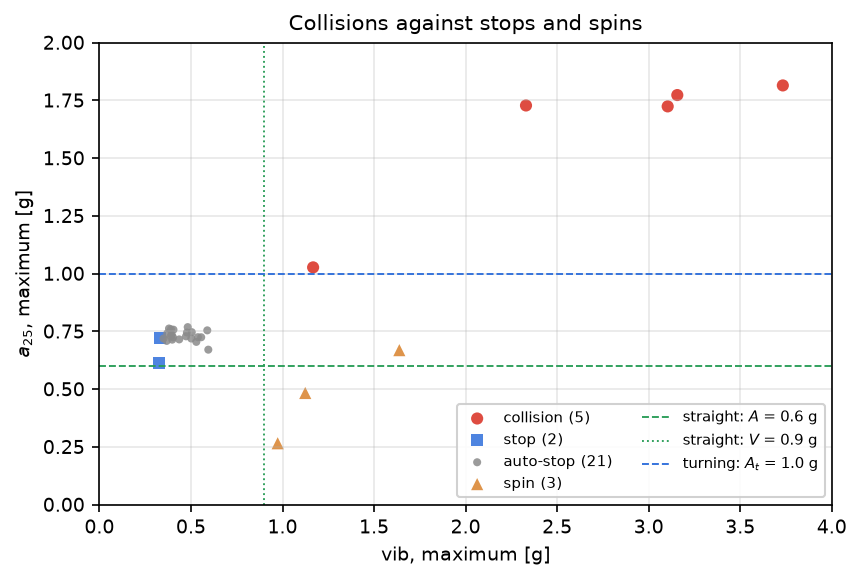
\includegraphics[width=0.92\linewidth]{figures/scatter.png}
  \caption{Event maxima of $\azf$ against $\vib$. Collisions (red) lie above both straight
    thresholds; stops and auto-stops lie above $A$ but outside the driving context; spins exceed
    $V$, which is not used while turning, and stay below $A_t$. Two of the five spins are not
    plotted; their recordings were not kept (0.38 and $0.27\g$ $\azf$).}
  \label{fig:scatter}
\end{figure}

Replaying every recording through the firmware code on a PC gives the same detections as the
analysis tool, with the same directions: front for the forward collisions, back-left for the two
backward collisions against the box and back for the shoe. Before the turning rule, spins raised
false alarms through $\vib$ (0.92 to $0.99\g$ against $V = 0.9\g$).

Figures~\ref{fig:collision} to~\ref{fig:spin} show the three cases in time. In the collision
the threshold is crossed at the contact, while the robot is driving (green); without the stop
mode the robot keeps pushing against the obstacle for another \SI{0.4}{\second}, which raises
$\vib$ to $3\g$. In the stop, $\azf$ crosses $A$ only after the driving phase has ended. In the
spin, $\vib$ crosses $V$ while $\azf$ stays far below $A_t$.

\begin{figure}[!htbp]
  \centering
  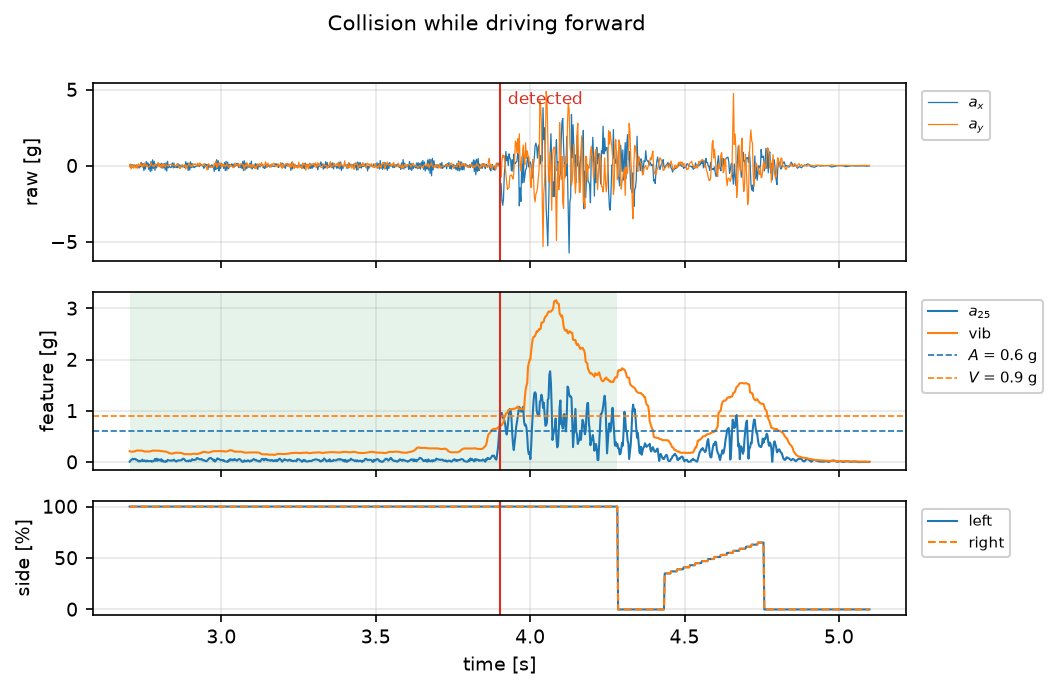
\includegraphics[width=\linewidth]{figures/collision.png}
  \caption{Collision while driving forward against a box. The red line marks the detection;
    green shading is the driving context.}
  \label{fig:collision}

  \vspace{1em}
  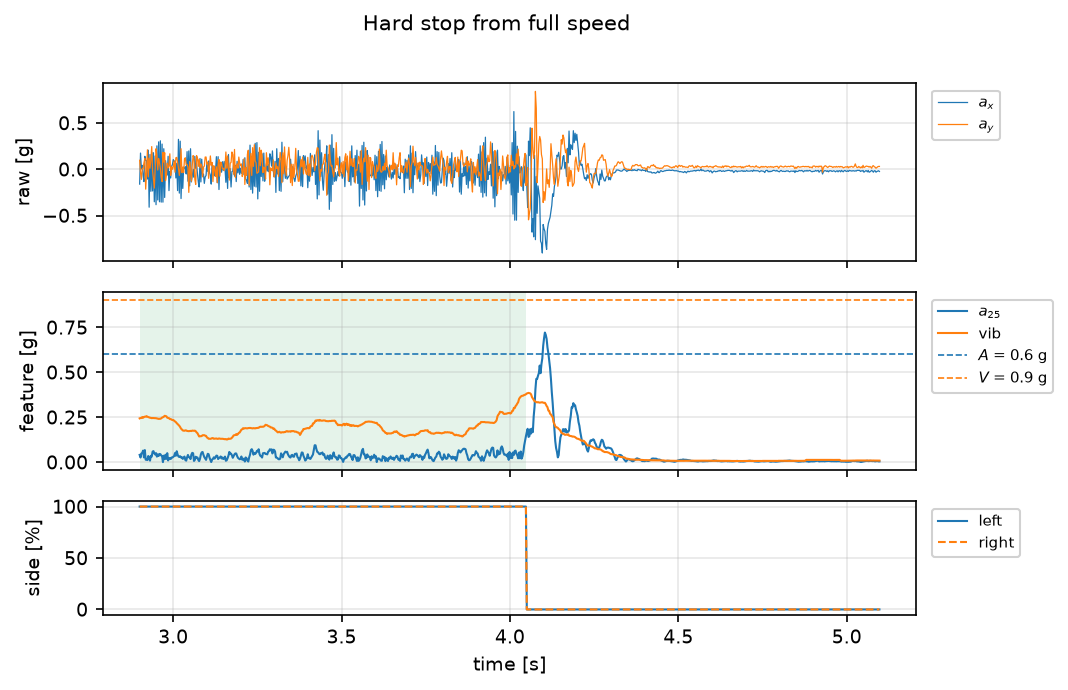
\includegraphics[width=\linewidth]{figures/stop.png}
  \caption{Hard stop from full speed. The jolt of $0.72\g$ $\azf$ follows the end of the driving
    phase and is therefore not a collision.}
  \label{fig:stop}
\end{figure}

\begin{figure}[!htbp]
  \centering
  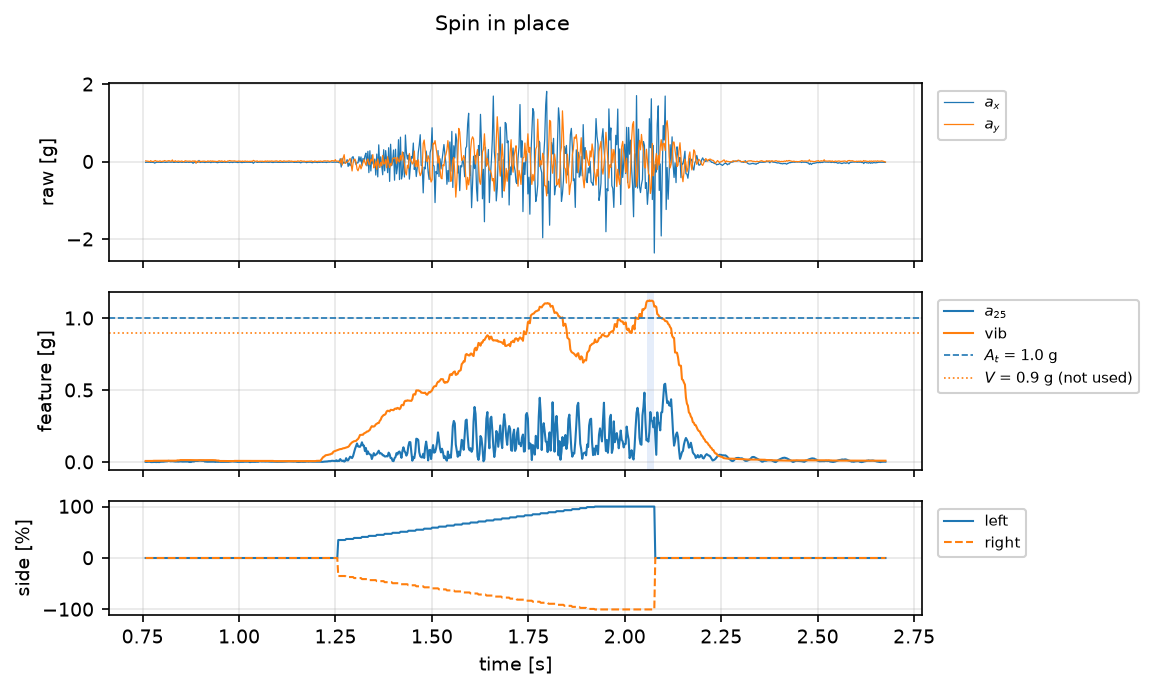
\includegraphics[width=\linewidth]{figures/spin.png}
  \caption{Spin in place. The vibration of the sliding wheels exceeds $V$; $\azf$ stays below
    $0.5\g$. The blue band is the turning context, reached \SI{0.8}{\second} after the start;
    this recording was made with firmware 0.8.0, which still stopped on the vibration.}
  \label{fig:spin}
\end{figure}

% ---------------------------------------------------------------------------------------
% Place the evaluation figures before the remaining sections.
\clearpage
\section{Limitations}

\begin{itemize}
  \item The evidence is one robot, one floor and 34 events. The thresholds are empirical and
    must be checked again with more data, other floors, speeds and loads.
  \item Collisions while turning have the thinnest margin: the softest collision reached
    $1.03\g$ against $A_t = 1.0\g$, and no collision during a turn has been recorded yet.
  \item A slow collision changes the velocity less and gives a smaller $\azf$; below about
    30\,\% speed a soft obstacle may go undetected.
  \item Collisions during the \SI{0.8}{\second} after a start or a reversal are not detected.
  \item Without wheel encoders the robot cannot tell that it stopped moving while its wheels
    still turn (pushing against an obstacle, stuck); odometry would add that signal.
  \item The sensor must be mounted rigidly; foam or a loose mount changes both features.
  \item Motor noise on the shared ground disturbs the I\textsuperscript{2}C bus (corrupted
    samples are discarded) and the Wi-Fi link; both need better wiring, not more filtering.
\end{itemize}

% ---------------------------------------------------------------------------------------
\section{Towards industrial AGVs}

The structure carries over, the numbers do not. A heavier vehicle has lower peaks and longer
contacts ($a_\text{peak} t_\text{contact} = \pi v$), different vibration and slower braking.
Relative criteria transfer better than fixed thresholds: an acceleration beyond what the brakes
and the tyre grip can produce ($\mu \gu$), a deceleration that does not match the command, and a
mismatch between wheel odometry and the integrated acceleration. IMU-based detection serves as a
diagnostic and logging layer; the protective function on an industrial AGV stays with certified
devices according to ISO~3691-4 and ISO~13849.

% ---------------------------------------------------------------------------------------
\appendix
\section{Constants}

{\small
\begin{longtable}{p{0.35\linewidth} p{0.27\linewidth} p{0.28\linewidth}}
  \hline
  Constant & Value & Where \\
  \hline
  \endhead
  Sample rate $f_s$              & \SI{400}{\hertz} (measured 392)   & \code{CONFIG\_ROBOT\_IMU\_RATE} \\
  Accelerometer resolution       & \SI{3.9}{\milli\gu}/count, $\pm16\g$ & \code{src/imu.c} \\
  Plausibility limit             & $\pm4096$ counts                  & \code{ADXL345\_MAX\_COUNTS} \\
  Accelerometer offsets          & 14, 0, \SI{151}{\milli\gu}       & \code{CONFIG\_ROBOT\_IMU\_}\allowbreak\code{ACCEL\_OFS\_*} \\
  Gyro bias: rest, average, reject & \SI{1}{\second}, 512 samples, \SI{3}{\degree\per\second} & \code{BIAS\_*} \\
  Tilt offset time constant      & 256 samples (\SI{0.64}{\second})  & \code{OFS\_SHIFT} = 8 \\
  $\azf$ window $N_s$            & 10 samples (\SI{25}{\milli\second}) & \code{WIN\_A25} \\
  $\vib$ window $N_v$            & 40 samples (\SI{100}{\milli\second}) & \code{WIN\_VIB} \\
  Warm-up                        & 100 samples                       & \code{WARMUP} \\
  Start and reversal exclusion   & \SI{0.8}{\second}                 & \code{START\_US} \\
  Thresholds $A$, $V$, $A_t$, $V_t$ & 0.6, 0.9, 1.0\,g, off         & Table~\ref{tab:thresholds} \\
  Direction samples              & 8 (\SI{20}{\milli\second})        & \code{DIR\_SAMPLES} \\
  Peak samples                   & 40 (\SI{100}{\milli\second})      & \code{PEAK\_SAMPLES} \\
  Monitor hold-off               & \SI{1}{\second}                   & \code{HOLDOFF\_US} \\
  IMU-only: $A'$, $V'$, $A'_t$   & 0.9, 0.9, 1.0\,g                 & \code{CONFIG\_ROBOT\_COLLISION\_}\allowbreak\code{IMU\_*} \\
  IMU-only: yaw window, $\Omega$, hold & \SI{250}{\milli\second}, \SI{10}{\degree\per\second}, \SI{0.5}{\second} & \code{WIN\_YAW}, \code{TURN\_HOLD\_US} \\
  Acting detector                & drive context                     & \code{CONFIG\_ROBOT\_COLLISION\_}\allowbreak\code{ACTING} \\
  Analysis: event merge, label window & \SI{0.3}{\second}, $-0.5$ to \SI{+3}{\second} & \code{tools/analyze.py} \\
  \hline
\end{longtable}
}

\end{document}
